\documentclass[]{article}
\usepackage{url}
\usepackage{hyperref}
\usepackage{tikz}				
\usepackage{xifthen}
\usepackage{pgfplots}
\usetikzlibrary{patterns}

\definecolor{p0}{HTML}{D7DFC0}
\definecolor{p1}{HTML}{AECFA2}
\definecolor{p2}{HTML}{82BC92}
\definecolor{p3}{HTML}{5FA38E}
\definecolor{p4}{HTML}{49848B}
\definecolor{p5}{HTML}{3F5F7F}
\definecolor{p6}{HTML}{383D65}
\definecolor{p7}{HTML}{2C1E3E}

\definecolor{r4}{HTML}{70488A}


\begin{document}
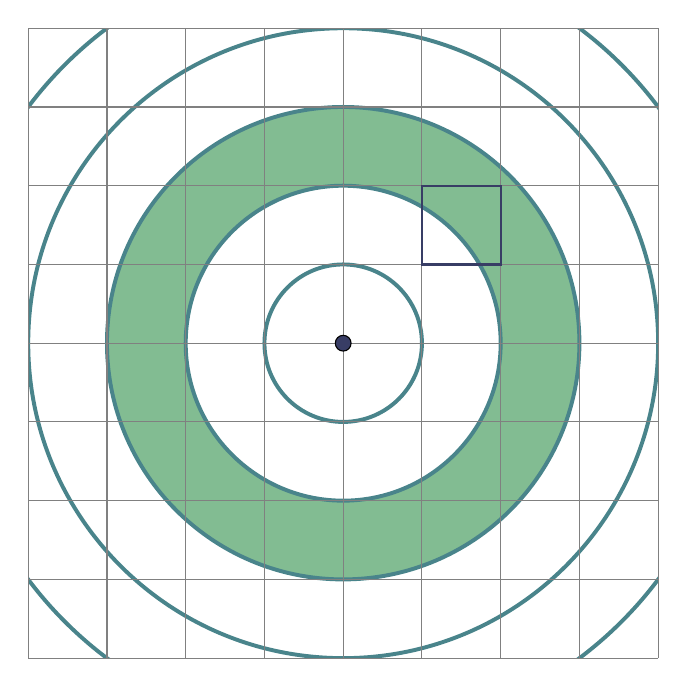
\begin{tikzpicture}
\begin{scope}
\clip (-4,-4) rectangle (4,4);
\draw[p4,line width=0.5mm, fill=p2] (0,0) circle (3cm);
\draw[p4,line width=0.5mm, fill=white] (0,0) circle (2cm);
\draw[p4,line width=0.5mm, fill=white] (0,0) circle (1cm);
\draw[p4,line width=0.5mm] (0,0) circle (4cm);
\draw[p4,line width=0.5mm] (0,0) circle (5cm);
\end{scope}
\draw[gray] (-4,-4) grid (4,4);
\draw[fill=p6] (0,0) circle (1mm);
\draw[thick, p6] (1,1) rectangle (2,2);
\end{tikzpicture}
\\*[1cm]
\indent

\begin{tikzpicture}
\draw[fill=p2] (8,8) rectangle (16,16);
\begin{scope}
\clip (8,8) rectangle (16,16);
\fill[thick, white] (0,0) circle (16);
\draw[thick, p4, line width=4mm] (0,0) circle (16);
\end{scope}
\draw[gray] (8,8) rectangle (16,16);

\end{tikzpicture}


\end{document}